\documentclass[portrait,final]{baposter}
%\documentclass[a4shrink,portrait,final]{baposter}
% Usa a4shrink for an a4 sized paper.

\tracingstats=2

\usepackage{verbatim} 
\usepackage{times}
\usepackage{calc}
\usepackage{graphicx}
\usepackage{amsmath}
\usepackage{amssymb}
\usepackage{relsize}
\usepackage{multirow}
\usepackage{bm}
\usepackage{epsfig}
\usepackage{graphicx}
\usepackage{multicol}
\usepackage{url}
\usepackage{cite}
\usepackage{pgfbaselayers}
\usepackage{algorithm,algorithmic}
\usepackage{tikz}
\usetikzlibrary{shapes,arrows}



\pgfdeclarelayer{background}
\pgfdeclarelayer{foreground}
\pgfsetlayers{background,main,foreground}
\usetikzlibrary{shapes,arrows}
\usepackage{helvet}
\usepackage{palatino}

\newcommand{\captionfont}{\footnotesize}

\selectcolormodel{cmyk}

\graphicspath{{images/}}

%%%%%%%%%%%%%%%%%%%%%%%%%%%%%%%%%%%%%%%%%%%%%%%%%%%%%%%%%%%%%%%%%%%%%%%%%%%%%%%%
%%%% Some math symbols used in the text
%%%%%%%%%%%%%%%%%%%%%%%%%%%%%%%%%%%%%%%%%%%%%%%%%%%%%%%%%%%%%%%%%%%%%%%%%%%%%%%%
% Format 
\newcommand{\Matrix}[1]{\begin{bmatrix} #1 \end{bmatrix}}
\newcommand{\Vector}[1]{\Matrix{#1}}
\newcommand*{\SET}[1]  {\ensuremath{\mathcal{#1}}}
\newcommand*{\MAT}[1]  {\ensuremath{\mathbf{#1}}}
\newcommand*{\VEC}[1]  {\ensuremath{\bm{#1}}}
\newcommand*{\CONST}[1]{\ensuremath{\mathit{#1}}}
\newcommand*{\norm}[1]{\mathopen\| #1 \mathclose\|}% use instead of $\|x\|$
\newcommand*{\abs}[1]{\mathopen| #1 \mathclose|}% use instead of $\|x\|$
\newcommand*{\absLR}[1]{\left| #1 \right|}% use instead of $\|x\|$

\def\norm#1{\mathopen\| #1 \mathclose\|}% use instead of $\|x\|$
\newcommand{\normLR}[1]{\left\| #1 \right\|}% use instead of $\|x\|$

%%%%%%%%%%%%%%%%%%%%%%%%%%%%%%%%%%%%%%%%%%%%%%%%%%%%%%%%%%%%%%%%%%%%%%%%%%%%%%%%
% Multicol Settings
%%%%%%%%%%%%%%%%%%%%%%%%%%%%%%%%%%%%%%%%%%%%%%%%%%%%%%%%%%%%%%%%%%%%%%%%%%%%%%%%
\setlength{\columnsep}{0.7em}
\setlength{\columnseprule}{0mm}


%%%%%%%%%%%%%%%%%%%%%%%%%%%%%%%%%%%%%%%%%%%%%%%%%%%%%%%%%%%%%%%%%%%%%%%%%%%%%%%%
% Save space in lists. Use this after the opening of the list
%%%%%%%%%%%%%%%%%%%%%%%%%%%%%%%%%%%%%%%%%%%%%%%%%%%%%%%%%%%%%%%%%%%%%%%%%%%%%%%%
\newcommand{\compresslist}{%
\setlength{\itemsep}{1pt}%
\setlength{\parskip}{0pt}%
\setlength{\parsep}{0pt}%
}


%%%%%%%%%%%%%%%%%%%%%%%%%%%%%%%%%%%%%%%%%%%%%%%%%%%%%%%%%%%%%%%%%%%%%%%%%%%%%%
%%% Begin of Document
%%%%%%%%%%%%%%%%%%%%%%%%%%%%%%%%%%%%%%%%%%%%%%%%%%%%%%%%%%%%%%%%%%%%%%%%%%%%%%

\begin{document}

%%%%%%%%%%%%%%%%%%%%%%%%%%%%%%%%%%%%%%%%%%%%%%%%%%%%%%%%%%%%%%%%%%%%%%%%%%%%%%
%%% Here starts the poster
%%%---------------------------------------------------------------------------
%%% Format it to your taste with the options
%%%%%%%%%%%%%%%%%%%%%%%%%%%%%%%%%%%%%%%%%%%%%%%%%%%%%%%%%%%%%%%%%%%%%%%%%%%%%%
% Define some colors
\definecolor{silver}{cmyk}{0,0,0,0.3}
\definecolor{yellow}{cmyk}{0,0,0.9,0.0}
\definecolor{reddishyellow}{cmyk}{0,0.22,1.0,0.0}
\definecolor{black}{cmyk}{0,0,0.0,1.0}
\definecolor{darkYellow}{cmyk}{0,0,1.0,0.5}
\definecolor{darkSilver}{cmyk}{0,0,0,0.1}

%\definecolor{lightyellow}{cmyk}{0,0,0.3,0.0}
\definecolor{lightyellow}{cmyk}{0,0,0.0,0.0}
\definecolor{lighteryellow}{cmyk}{0,0,0.0,0.0}
%\definecolor{lighteryellow}{cmyk}{0,0,0.1,0.0}
\definecolor{lighteryellow}{cmyk}{0,0,0.0,0.0}
\definecolor{lightestyellow}{cmyk}{0,0,0.0,0.0}

%%
\typeout{Poster Starts}
%\background{
%  \begin{tikzpicture}[remember picture,overlay]%
%    \draw (current page.north west)+(-2em,2em) node[anchor=north west] {\includegraphics[height=1.1\textheight]{silhouettes_background}};
%  \end{tikzpicture}%
%}

\newlength{\leftimgwidth}
\begin{poster}%
  % Poster Options
  {
  % Show grid to help with alignment
  grid=no,
  % Column spacing
  colspacing=1em,
 % columns=2,
  % Color style
  bgColorOne=lighteryellow,
  bgColorTwo=lightestyellow,
  borderColor=reddishyellow,
  headerColorOne=yellow,
  headerColorTwo=reddishyellow,
  headerFontColor=black,
  boxColorOne=lightyellow,
  boxColorTwo=black,
  % Format of textbox
  textborder=roundedleft,
  % Format of text header
  eyecatcher=yes,
  headerborder=open,
  headerheight=0.1\textheight,
  headershape=roundedright,
  headershade=plain,
  headerfont=\large\textsf, %Sans Serif
  boxshade=plain,
%  background=shade-tb,
  background=plain,
  linewidth=2pt
  }
  % Eye Catcher
  {
\includegraphics[height=5em]{logopsi}} % No eye catcher for this poster. (eyecatcher=no above). If an eye catcher is present, the title is centered between eye-catcher and logo.
  % Title
  {\sf %Sans Serif
  %\bf% Serif
  A Field Emission and Secondary\\[3mm] Emission Model in OPAL}
  % Authors
  {\sf %Sans Serif
  % Serif
  \vspace{1em}C.Wang, A. Adelmann, Y. Ineichen, PSI, Villigen, Switzerland \\
 
 
  }
   % University logo
  {% The makebox allows the title to flow into the logo, this is a hack because of the L shaped logo.
    \makebox[8em][r]{%
      \begin{minipage}{12em}
        \hfill
        %
\includegraphics[height=4em]{psilogo}
        %\includegraphics[height=7.0em]{logo}
      \end{minipage}
    }
  }

  \tikzstyle{light shaded}=[top color=baposterBGtwo!30!white,bottom color=baposterBGone!30!white,shading=axis,shading angle=30]

  % Width of left inset image
     \setlength{\leftimgwidth}{0.78em+8.0em}

%%%%%%%%%%%%%%%%%%%%%%%%%%%%%%%%%%%%%%%%%%%%%%%%%%%%%%%%%%%%%%%%%%%%%%%%%%%%%%
%%% Now define the boxes that make up the poster
%%%---------------------------------------------------------------------------
%%% Each box has a name and can be placed absolutely or relatively.
%%% The only inconvenience is that you can only specify a relative position 
%%% towards an already declared box. So if you have a box attached to the 
%%% bottom, one to the top and a third one which should be in between, you 
%%% have to specify the top and bottom boxes before you specify the middle 
%%% box.
%%%%%%%%%%%%%%%%%%%%%%%%%%%%%%%%%%%%%%%%%%%%%%%%%%%%%%%%%%%%%%%%%%%%%%%%%%%%%%
    %
    % A coloured circle useful as a bullet with an adjustably strong filling
    \newcommand{\colouredcircle}[1]{%
      \tikz{\useasboundingbox (-0.2em,-0.32em) rectangle(0.2em,0.32em); \draw[draw=black,fill=baposterBGone!80!black!#1!white,line width=0.03em] (0,0) circle(0.18em);}}

%%%%%%%%%%%%%%%%%%%%%%%%%%%%%%%%%%%%%%%%%%%%%%%%%%%%%%%%%%%%%%%%%%%%%%%%%%%%%%
  \headerbox{Motivation and Introduction}{name=abstract,column=0,row=0,span=3}{
%%%%%%%%%%%%%%%%%%%%%%%%%%%%%%%%%%%%%%%%%%%%%%%%%%%%%%%%%%%%%%%%%%%%%%%%%%%%%%
\sf  Dark current and multipacting phenomena have been observed in various RF structures
of accelerators. These phenomena are usually harmful to the equipment and to
the beam quality, as they will cause galvanic etching on the surface of the
cavity and thus cause RF breakdown. Our efforts to extend OPAL\cite{OP} to get a
feasible tool to perform large scale simulations. Such a tool would allow
rigorous analysis and understanding of these phenomena and hopefully leads
to methods how these situations can be prevented or diminished. To achieve these
goals, we first add a particle-boundary collision test model into OPAL to
facilitate the particle searching during the particle tracking process. A
Fowler-Nordheim field emission model and surface physics models including a
phenomenological secondary emission model complete the particle matter
interaction model. Space charge of emitted electrons is considered by the
Child-Langmuir law. An iterative solver\cite{SV} for space charge handling
complicated boundary geometries is currently under development. A code benchmark of the
secondary model in OPAL and visualization of simulation results are also shown
here.
\vspace{0.3em}
 }

%%%%%%%%%%%%%%%%%%%%%%%%%%%%%%%%%%%%%%%%%%%%%%%%%%%%%%%%%%%%%%%%%%%%%%%%%%%%%%
  \headerbox{Particle-Boundary Collision Test Model}{name=model,column=0,span=2,below=abstract}{
%%%%%%%%%%%%%%%%%%%%%%%%%%%%%%%%%%%%%%%%%%%%%%%%%%%%%%%%%%%%%%%%%%%%%%%%%%%%%%

\sf Testing particle-boundary collisions is crucial to both dark current and
multipacting simulation. We need an efficient way to distinguish between dark
current particles which potentially reach the beam diagnostic equipment (e.g. a
screen) and those hitting the surface of beam line elements consequently cause
multiplication.

Coming up with an efficient particle-boundary collision test in a 3D geometry is
challenging, since the 3D geometry is hard to be parameterized by simple
functions unlike in the 2D case. We use a oriented triangulated surface mesh to
represent the complicated 3D geometry and use 3D line segment-triangle
intersection (LSTI) tests\cite{LT,FA} to find particle-boundary collisions.\\

%\\\mbox{\hspace{0.3\linewidth}\rule{0.4\linewidth}{1pt}\hspace{0.3\linewidth}}\\
      \begin{tabular}{cc}
        \hspace{-0.5em}\scalebox{1.035}{\scalebox{0.7}{
\begin{tikzpicture}
\usetikzlibrary{arrows}
\draw [->,black,-latex] (-1.5,0) -- (1.5,0);
\draw [->,black,-latex] (-1.5,0) -- (-1.5,2);
\draw (1.5,0) -- (0.0,2);
\draw  [<-,black,latex-](0.0,2) -- (-1.5,0.0);
\draw [->,black,-latex,dashed] (-1.5,0) -- (0.5,0.5);
\node[below] (w) at (-0.15,0.5) {$\vec{w}$};
\draw[dashed] (0.5,0.5) -- (-1.18,0.5);
\draw[dashed] (0.5,0.5) -- (0.01,0.0);
\node[above] (ti) at (-1.18,0.5) {$t_i$};
\node[below] (si) at (0.01,0.0) {$s_i$};
\node[above] (t0) at (-1.7,0.) {$\mathbf{t_0}$};
\node[right] (t1) at (1.5,0) {$\mathbf{t_1}$};
\node[above] (t2) at (0.0,2.0) {$\mathbf{t_2}$};
\node[above] (n) at (-1.5,2) {$\vec{n}$};
\node[above] (v) at (-0.5,1.5) {$\vec{v}$};
\node[below] (u) at (1.2,0.0) {$\vec{u}$};
\path[draw=black,fill=black] (0.0,2.0) circle (2pt);
\path[draw=black,fill=black] (1.5,0.0) circle (2pt);
\path[draw=black,fill=black] (-1.5,0.0) circle (2pt);
\draw (-3.5,-1) -- (2.5,-1);
\draw (2.5,-1) -- (5,3);
\draw (0,3) -- (5,3);
\draw (-3.5,-1) -- (0,3);
\draw (0.5,0.5) -- (1.6,5);
\path[draw=black] (0.5,0.5) circle (2pt);
\node[above] (I) at (0.5,0.5) {$\mathbf{I}$};
\node[right] (x0) at (1.6,5) {$\mathbf{x_0}$};
\draw[dashed] (0.5,0.5) -- (-0.1,-1.9);
\node[right] (x1) at (0.0,-1.9) {$\mathbf{x_1}$};
\node[right] (ri) at (1,2.5) {$r_i$};
\path[draw=black,fill=black] (-0.1,-1.9) circle (2pt);
\path[draw=black,fill=black] (1.6,5) circle (2pt);
\end{tikzpicture}
}} & \hspace{5em}
        %\hspace{2em}\scalebox{0.9}{\includegraphics[height=40em]{algorithm.pdf}} &
            %\hspace{0.5em}\scalebox{1.}{\input{und_mncg}}
        %\hspace{1.5em}\scalebox{1.}{\epsfig{figure=2d_grid,height=100em}}
        \hspace{-5.5em}\scalebox{0.835}{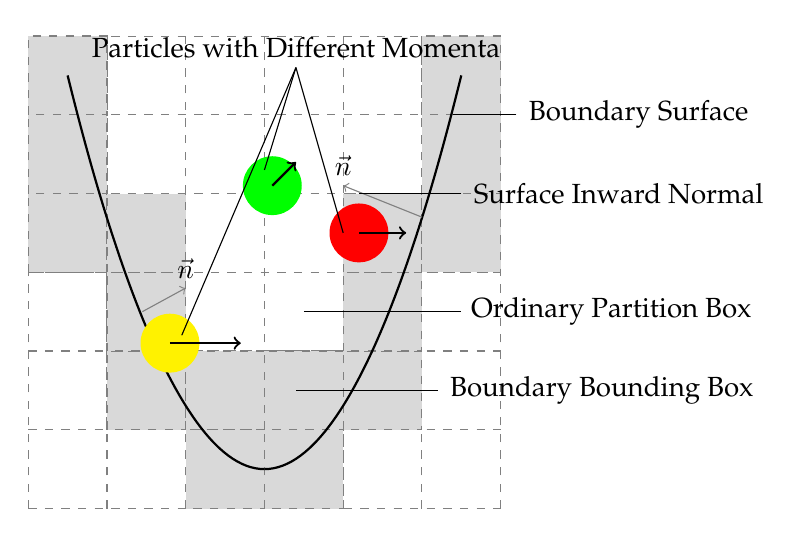
\begin{tikzpicture}

\draw[step=1cm,gray,dashed,fill=white] (-3,0) grid (3,6);

\draw[step=1cm,gray,dashed,fill=gray!30] (-3,3) rectangle (-2,4); 
\draw[step=1cm,gray,dashed,fill=gray!30] (-2,1) rectangle (-1,2); 
\draw[step=1cm,gray,dashed,fill=gray!30] (-2,2) rectangle (-1,3); 
\draw[step=1cm,gray,dashed,fill=gray!30] (-2,3) rectangle (-1,4);
\draw[step=1cm,gray,dashed,fill=gray!30] (-1,1) rectangle (0,2);
\draw[step=1cm,gray,dashed,fill=gray!30] (-1,0) rectangle (0,1);
\draw[step=1cm,gray,dashed,fill=gray!30] (0,0) rectangle (1,1);
\draw[step=1cm,gray,dashed,fill=gray!30] (0,1) rectangle (1,2);
\draw[step=1cm,gray,dashed,fill=gray!30] (1,1) rectangle (2,2);
\draw[step=1cm,gray,dashed,fill=gray!30] (1,2) rectangle (2,3); 
\draw[step=1cm,gray,dashed,fill=gray!30] (1,3) rectangle (2,4);
\draw[step=1cm,gray,dashed,fill=gray!30] (2,3) rectangle (3,4);
\draw[step=1cm,gray,dashed,fill=gray!30] (-3,4) rectangle (-2,5);
\draw[step=1cm,gray,dashed,fill=gray!30] (-3,5) rectangle (-2,6);
\draw[step=1cm,gray,dashed,fill=gray!30] (2,4) rectangle (3,5);
\draw[step=1cm,gray,dashed,fill=gray!30] (2,5) rectangle (3,6);   
\draw[black, thick] (0.,0.5) parabola  ( 2.5,5.5); 
\draw[black, thick] (0.,0.5) parabola  ( -2.5,5.5);
\draw [->,gray] (-1.55,2.5) -- (-1,2.8);
\node[above] (n) at (-1,2.8) {$\vec{n}$};
\draw [<-,gray] (1.0,4.1) -- (2,3.7);
\node[above] (n) at (1,4.1) {$\vec{n}$};
%\tikz[label distance=4mm]
\draw (-1.2,2.1) node[circle,fill=yellow, yellow]{no};
\draw [->,thick] (-1.2,2.1) -- (-0.3,2.1);
\draw (0.1,4.1) node[circle,fill=green, green]{no};
\draw [->,thick] (0.1,4.1) -- (0.4,4.4);
\draw (1.2,3.5) node[circle, fill=red, red]{no};
\draw [<-,thick] (1.8,3.5) -- (1.2,3.5);
\draw [-,black] (3.2,5) -- (2.4,5);
\draw (3.2,5) node[above=0pt, right=1pt] {Boundary Surface};
\draw [-,black] (2.2,1.5) -- (0.4,1.5);
\draw (2.2,1.5) node[above=0pt, right=1pt] {Boundary Bounding Box};
\draw [-,black] (2.5,4) -- (1.2,4);
\draw (2.5,4) node[above=0pt, right=1pt] {Surface Inward Normal};
\draw [-,black] (0.4,5.6) -- (1.0,3.5);
\draw [-,black] (0.4,5.6) -- (0,4.3);
\draw [-,black] (0.4,5.6) -- (-1.05,2.2);
\draw (0.4,5.6) node[above=0.1pt] {Particles with Different Momenta};
\draw [-,black] (0.5,2.5) -- (2.5,2.5);
\draw (2.5,2.5) node[above=0pt, right=0pt] {Ordinary Partition Box};
\end{tikzpicture}}
      \end{tabular}\\
      
\sf Since the number of triangles $M$ and the number of simulated particles $N$ are both in the magnitude of hundreds of thousand to millions, the number of LSTI tests in single time step without a early rejection strategy will be $M \times N$, i.e., at least $10^{10}$ per time step. This is beyond existing and future computing capabilities. \\
\sf The early rejection strategies are sketched on the right in the figure
above. For each particle, we consider both its position and its momenta
direction. The direction of momenta and norm determines if a particle is tested
for collision. In the example above we only will perform the LSTI with the
red particle.

      \vspace{0.3em}
    }
%%%%%%%%%%%%%%%%%%%%%%%%%%%%%%%%%%%%%%%%%%%%%%%%%%%%%%%%%%%%%%%%%%%%%%%%%%%%%%
  \headerbox{\sf Field Emission Model}{name=FN,column=2,span=1,below=abstract}{
%%%%%%%%%%%%%%%%%%%%%%%%%%%%%%%%%%%%%%%%%%%%%%%%%%%%%%%%%%%%%%%%%%%%%%%%%%%%%%
\sf Field emission is a major source of both dark current particles and primary 
incident particles in secondary emission. The Fowler-Nordheim (FN) model
\cite{BC,FN} is used to predict the emitted current density
reads:
\begin{equation*}\label{eq:units}
    J(\mathbf{r},t) = \frac{A(\beta E)^2}{\varphi t(y)^2}\exp{\left(\frac{-B v(y)\varphi^{3/2}}{\beta E}\right)} [\hbox{A/$m^2$}] \text{.}
\end{equation*}

\sf In some rare occasion where the normal component of the electric field is
high enough the field emission current density will be limited by space charge
effects\cite{BC}. Currently space charge is modelled by the 1D Child-Langmuir 
law
\begin{align*}
J(\mathbf{r},t) & =\frac{4\varepsilon_0}{9}\sqrt{2\frac{e}{m}}\left(\frac{V^{3/2}}{d^2}\right)\notag\\
 & =\frac{4\varepsilon_0}{9}\sqrt{2\frac{e}{m}}\left(\frac{E^{3/2}}{d^{1/2}}\right) [\hbox{A/$m^2$}]
\end{align*}
introducing the space charge limited field emission.

\sf A multigrid preconditioned iterative space charge solver\cite{SV} has
already been implemented in OPAL. Applying the iterative space charge solver in
this setting is still working in progress.

\vspace{0.5em}
  }

%%%%%%%%%%%%%%%%%%%%%%%%%%%%%%%%%%%%%%%%%%%%%%%%%%%%%%%%%%%%%%%%%%%%%%%%%%%%%%
  \headerbox{\sf Secondary Emission Model}{name=se,column=0,span=1,above=bottom}{
%%%%%%%%%%%%%%%%%%%%%%%%%%%%%%%%%%%%%%%%%%%%%%%%%%%%%%%%%%%%%%%%%%%%%%%%%%%%%%
\sf The secondary emission model is based on the phenomenological model
developed by M. A. Furman and M. Pivi\cite{SE}. \\

\begin{center}
 \begin{tabular}{cc}
        \hspace{1em}\scalebox{0.82}{/Users/adelmann/svnwork/adelmann/papers/figures/Latex-Figures/Incident.tikz} 
 \end{tabular} \\
 \tiny{Model of backscattered, redifused and true secondary electrons.}
\end{center}
%
\begin{center}
 \begin{tabular}{cc}
        \hspace{1em}\scalebox{0.655}{%\usepackage[latin1]{inputenc}
%\usepackage{tikz}
%\usetikzlibrary{shapes,arrows}

%<
%\usepackage{verbatim}
%\usepackage[active,tightpage]{preview}
%\PreviewEnvironment{tikzpicture}
%\setlength\PreviewBorder{5pt}%
%



% Define block styles
\tikzstyle{decision} = [draw,diamond, fill=blue!20, 
    text width=4.5em, text badly centered, node distance=2.2cm, inner sep=0pt]
\tikzstyle{block} = [draw,rectangle, fill=blue!20, 
    text width=7.5em, text badly centered, inner sep=3pt, rounded corners, minimum height=4em]
\tikzstyle{line} = [draw, -latex']
\tikzstyle{cloud} = [draw, \ellipse,fill=red!20, node distance=2.2cm,
    minimum height=2em]
\tikzstyle{every node}=[font=\small]
\scalebox{0.75}{
\begin{tikzpicture}[node distance = 2.2cm, auto, every node/.style={anchor=base,font=\small}]
    % Place nodes
    \node [block] (incident) {Incident $E_0$, $\theta_0$};
   % \node [cloud, left of=incident] (expert) {expert};
   % \node [cloud, right of=incident] (system) {system};
    \node [block, below of=incident, node distance=2.2cm] (yield) {Compute $\delta_e(E_0,\theta_0)$, $\delta_r(E_0,\theta_0)$, $\delta_{ts}(E_0,\theta_0)$};
    \node [block, below of=yield, node distance=2.2cm] (probability) {Compute $P_n, n=0,1,...,M$};
    \node [block, below of=probability, node distance=2.5cm] (secondaryNum) {Random integer $n$ with probability distribution $\{P_n\}$};
    \node [decision, right of=incident, node distance=3.5cm] (decide) {$n=0$?};
    \node [block, right of=decide, node distance=3.5cm] (zero) {Delete the incident electron};
    \node [decision, below of=decide, node distance=3.0cm] (decide1) {$n=1$?};
    \node [block, right of=decide1, node distance=3.5cm] (one) {Emitted energy $E\in[0,E_0]$ with PDF $f_{1,e}+f_{1,r}+f_{1,ts}$ };	\node [block, below of=decide1, node distance=3.5cm] (ts) {Emitted energy $E_k\in[0,E_0]$, $k=1,...,n$ with PDF $f_{n,ts}$ };
    \node [block, below of=one, node distance=3.5cm] (angle) {Generate $\theta_k\in[0,\pi/2]$, with PDF $cos^{\alpha}$; and $\phi_k\in[0,2\pi]$, $k=1,...,n$. Calc momenta accordingly. };
    % Draw edges
    \path [line] (incident) -- (yield);
    \path [line] (yield) -- (probability);
    \path [line] (probability) --  (secondaryNum);		
   % \path [line] (probability) -- (secondaryNum);
   % \path [line] (decide) -- node [near start] {$No$} (secondaryNum);
    \draw[->] (secondaryNum) -| +(1.8,3) |- (decide);
    %\path [line] (decide) -- node [near start,above] {yes} (zero);
    \draw[->] (decide) -- node [midway,above=2pt] {yes} (zero);	
    \path [line] (decide) -- node [midway,right=2pt] {no} (decide1);
    \path [line] (decide1) -- node [midway,above=2pt] {yes} (one);
    \path [line] (decide1) -- node [midway,right=2pt] {no} (ts);
    \path [line] (ts) -- (angle);

    \path [line] (one) -- (angle);
    \path [line] (zero) -- +(0,1.5)-| node [near start,above=2pt] {Next event} (incident);
    \path [line] (angle) -- +(0,-2.)--  node [midway,above=2pt] {Next event} (-2,-8.65) |- (incident) ;
 %\path [line] (secondaryNum) -|- (decide);
  %  \path [line] (decide) -- node {no}(stop);
   % \path [line,dashed] (expert) -- (incident);
  %  \path [line,dashed] (system) -- (incident);
   % \path [line,dashed] (system) |- (probability);
\end{tikzpicture}
}
} 
  \end{tabular} \\
  \tiny{Flow diagram for the computational procedure.}
\end{center}
}

%%%%%%%%%%%%%%%%%%%%%%%%%%%%%%%%%%%%%%%%%%%%%%%%%%%%%%%%%%%%%%%%%%%%%%%%%%%%%%
  \headerbox{\sf Future Work}{name=references,column=2,below=FN}{
%%%%%%%%%%%%%%%%%%%%%%%%%%%%%%%%%%%%%%%%%%%%%%%%%%%%%%%%%%%%%%%%%%%%%%%%%%%%%%
 \sf
      \begin{itemize}
        \item Validation of the FN-Model (analytic?)
        \item Use the iterative space charge solver\cite{SV} for increased accuracy
        \item Multipacting studies of RF structures in Cyclotrons (PSI \& CIAE)
        \item Improve the parallel efficiency of the particle-boundary collision
        test model 
      \end{itemize}
 }





%%%%%%%%%%%%%%%%%%%%%%%%%%%%%%%%%%%%%%%%%%%%%%%%%%%%%%%%%%%%%%%%%%%%%%%%%%%%%%
  \headerbox{\sf References}{name=references,column=2,above=bottom}{
%%%%%%%%%%%%%%%%%%%%%%%%%%%%%%%%%%%%%%%%%%%%%%%%%%%%%%%%%%%%%%%%%%%%%%%%%%%%%%
  
    \smaller
    \vspace{-0.4em}
    \bibliographystyle{ieee}
    \renewcommand{\section}[2]{\vskip 0.05em}
      \begin{thebibliography}{1}\itemsep=-0.01em
      \setlength{\baselineskip}{0.4em}
    \bibitem{OP}\sf A. Adelmann et.al ,
      The OPAL (Object Oriented Parallel Accelerator Library) 
              Framework, Paul Scherrer Institut, PSI-PR-08-02, 2008-2010
\bibitem{SV}\sf A. Adelmann, P. Arbenz and Y. Ineichen, 
J. Comp. Phys, 229 (12): 4554-4566 (2010)
%\bibitem{DE}\sf J. H. Han, PhD Thesis, Desy, 2005 Available Online on \url{http://www-library.desy.de/preparch/desy/thesis/desy-thesis-05-045.pdf}
%\bibitem{CY}\sf P. K. Sigg, Reliability of High Beam Power Cyclotron RF-Systems at PSI, Proceedings of the Workshop on Utilization and Reliability of High Power Proton Accelerators: Aix-en-Provence, France, 22-24 November 1999. Available Online on: \url{http://rf.web.psi.ch/files/proceedings/1998/JAERI98/PaperNEA98.pdf}.
\bibitem{FA}\sf T. M\"oller and B. Trumbore,
 ACM SIGGRAPH 2005 Courses, July 31-August 04, 2005, Los Angeles, California   [doi:10.1145/1198555.1198746] 
\bibitem{LT}\sf D. Sunday,
 Available Online on: \url{http://softsurfer.com/Archive/algorithm_0105/algorithm_0105.htm}
\bibitem{BC}\sf Y. Feng and J. P. Verboncoeur,
Phys.Plasmas 13, 073105 (2006)
\bibitem{FN}\sf R. H. Fowler and L. Nordheim, 
Proc. R. Soc. London, Ser. A 119, 173 (1928)

\bibitem{SE}\sf M. A. Furman and M. T. F. Pivi,  
Phys. Rev. ST Accel. Beams 5, 124404 (2002)
\bibitem{TX}\sf TxPhysics Users Manual, \url{http://txphysics.txcorp.com}
%\bibitem{PR}\sf A. Henderson, ParaView Guide, A Parallel Visualization Application. Kitware Inc., 2007. \url{http://www.kitware.com/products/paraview.html}
     
      \end{thebibliography}
 }

%%%%%%%%%%%%%%%%%%%%%%%%%%%%%%%%%%%%%%%%%%%%%%%%%%%%%%%%%%%%%%%%%%%%%%%%%%%%%%
  \headerbox{\sf Model Benchmark and Visualization}{name=bench,column=1,span=1,above=bottom}{
  \vspace{-1mm}
%%%%%%%%%%%%%%%%%%%%%%%%%%%%%%%%%%%%%%%%%%%%%%%%%%%%%%%%%%%%%%%%%%%%%%%%%%%%%%
\sf We have validated the secondary emission model by a code to code comparison with the TxPhysics library \cite{TX}.
%
 \begin{tabular}{cc}
        \hspace{0.2em}\scalebox{1}{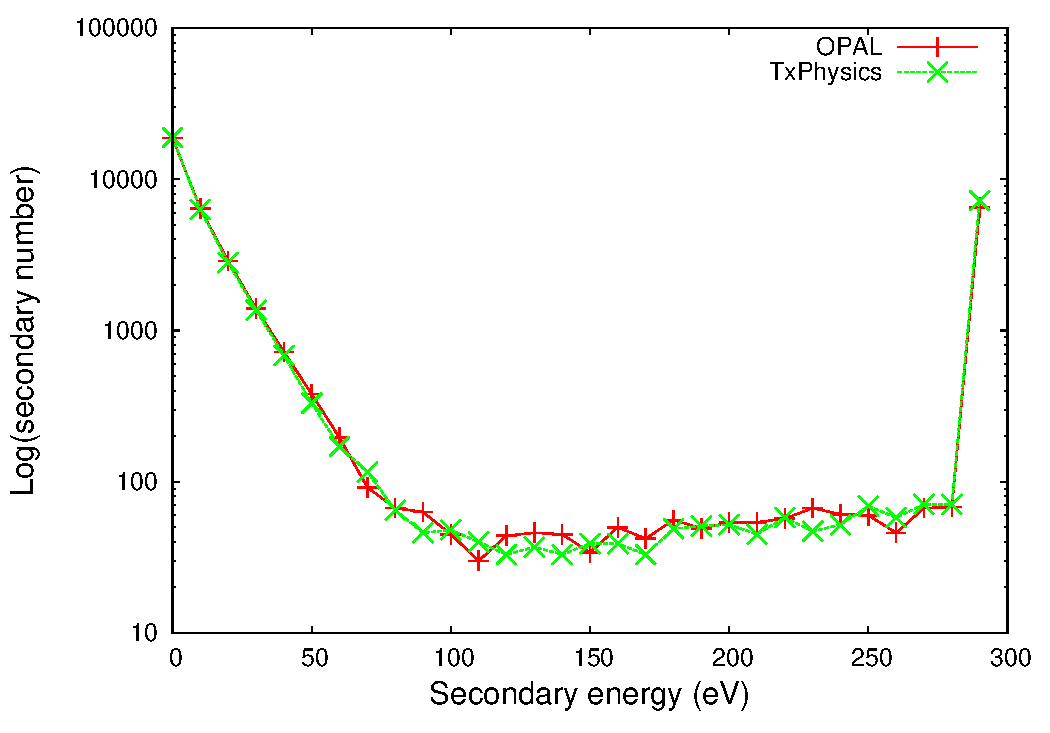
\includegraphics[width=0.92\textwidth]{code_comparison.pdf}} 
 \end{tabular}\\

%
\sf The boundary geometry and particles phase space are dumped into VTK files.
%
\begin{center}
\begin{tabular}{cc}
        \hspace{2em}\scalebox{1}{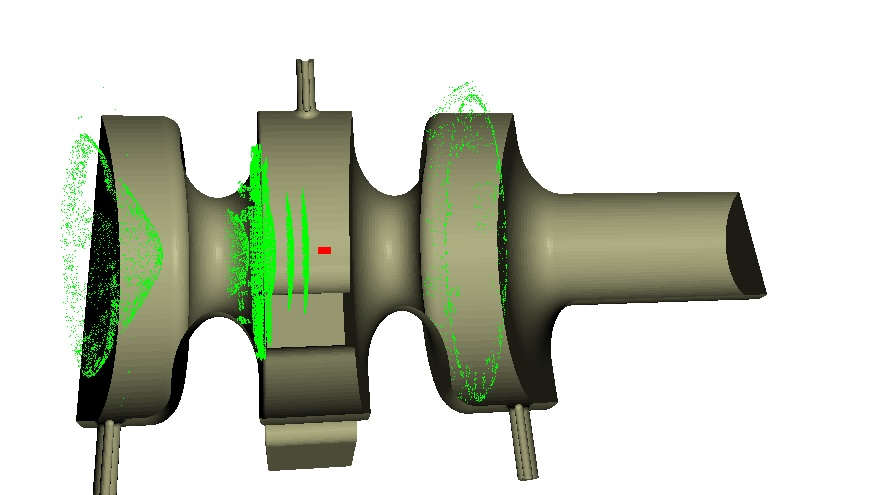
\includegraphics[width=0.715\textwidth]{newgun.jpg}} 
 \end{tabular}\\
    \tiny{Dark current simulation of the PSI XFEL gun. Red particles are bunch particles and green particles the dark current.}
 \end{center}
}
%
\end{poster}%
\end{document}
